\chapter{自発的超対称性の破れと最初の\texorpdfstring{\(SU(5)\)}{SU(5)}多重項}

\lectureoverview{対称性の破れは、まずスペクトルに関する目に見える事実として現れる。回転不変な原子は角運動量準位が縮退しているが、磁場はそれらを分裂させる。次に強磁性体は、方程式がある対称性を保っていても真空はそれを保たないという、より微妙な教訓を与える。ギャップのないマグノン、条件\(J|0\rangle\neq0\)、そして非零の秩序変数は、同じ現象の三つの記述である。このパターンをカイラルな超対称場の理論に持ち込み、補助場\(F\)を消去してスカラーポテンシャル\(V=|W'|^2\)を導き、超対称な真空と\(F\)を破る真空とを区別する。その結果得られる真空エネルギー、ボソン--フェルミオン分裂、ゴールドスティーノ、隠れたセクター、そして超ヒッグス機構が超対称性の議論を完結させる。最後の部分は話題を変えて大統一を開く。\(SU(3)\times SU(2)\times U(1)\)は\(SU(5)\)の中にブロックごとに埋め込まれ、その最初の物質多重項はレプトン二重項と三つの反ダウンクォークを組み合わせる。}

\section{スペクトルはその対称性を記憶する}

原子から始める目的は、単に初等的な量子力学を復習することではない。エネルギー準位と粒子の質量は同じ種類のスペクトルデータである。ある対称性が原子の準位の一致を強制するなら、その破れはそれらの準位を分裂させうる。場の理論における対応する主張は、粒子多重項のメンバーが異なる質量を獲得しうるということである。

原子状態が、スピンと軌道の寄与の両方を含む全角運動量\(j\)をもつとしよう。任意に選んだ軸に対して、
\begin{equation}
J_z|j,m\rangle=m\hbar|j,m\rangle,
\qquad
m=-j,-j+1,\ldots,j,
\end{equation}
であるから、\(2j+1\)個の状態がある。よく知られた教科書の矢印は、角運動量ベクトルが文字通り\(2j+1\)通りの可能な空間方向しかもたないと言っていると読むべきではない。量子化されているのは、選んだ軸に沿ったその成分である。

空っぽで回転不変な空間では、その軸を選び取る物理的な理由はない。回転はスピン\(j\)多重項内の状態を混ぜ合わせ、ハミルトニアンの不変性は
\begin{equation}
[H,\mathbf J]=0,
\qquad
E_{j,-j}=E_{j,-j+1}=\cdots=E_{j,j}.
\label{eq:l9-degeneracy}
\end{equation}
を意味する。

\begin{classroomqa}
\audiencequestion{原子全体を回転させてもそのエネルギーを変えられないと、対称性は何を言っているのか。\lecturetimestamp{00:05:53}}
\lecturerresponse{回転対称性である。回転は物理系を変えることなく角運動量のある向きを別の向きへ移すので、\(2j+1\)個の状態はすべて同じエネルギーをもつ。}
\end{classroomqa}

次に磁場\(\mathbf B=B\hat{\mathbf z}\)を加える。相互作用
\begin{equation}
H_B=-\boldsymbol{\mu}\cdot\mathbf B
\end{equation}
は磁場に平行な成分を区別する。模式的には、
\begin{equation}
\Delta E_m\propto mB.
\label{eq:l9-zeeman}
\end{equation}
であり、弱磁場では異なる\(m\)をもつ準位が線形に分離し、それらの間の遷移がスペクトル線を分裂させる。

\begin{classroomqa}
\audiencequestion{磁場中での原子準位の分裂は何と呼ばれるか。\lecturetimestamp{00:07:13}}
\lecturerresponse{ゼーマン効果である。これは議論全体の原型である。対称性によって縮退させられた準位は、背景がその対称性を破ると分離する。}
\end{classroomqa}

\begin{center}
\begin{tikzpicture}[x=1.05cm,y=0.75cm,>=Latex]
  \draw[thick] (-3,0) -- (-1,0);
  \node[left] at (-3,0) {\(B=0\)};
  \foreach \y/\m in {-1.2/-1,-0.4/0,0.4/1,1.2/2} {
    \draw[thick,teal!70!black] (1,\y) -- (3,\y);
    \node[right] at (3,\y) {\(m=\m\)};
  }
  \draw[->,thick] (-0.5,0) -- (0.6,0);
  \node[above] at (0.05,0) {\(\mathbf B\neq0\)};
\end{tikzpicture}
\end{center}

\section{強磁性体：対称な法則、非対称な真空}

強磁性体の簡単な微視的描像では、各サイトに小さな磁気モーメントを割り当てる。隣り合うモーメントが平行になることでエネルギーを下げるなら、低温相は強磁性である。反平行の整列が好まれるなら、結果は反強磁性である。強い熱的ゆらぎや量子的ゆらぎは、代わりに正味の磁化を洗い流しうる。

強磁性体が世界を満たし、一様に整列した状態に落ち着いたとしよう。その内部磁場は、外部から加えられた磁場とちょうど同じように原子の準位を分裂させる。しかし決定的な違いがある。根底にある相互作用は北や東やその他の方向を好まない。一様に回転させた配置はすべて同じエネルギーをもつ：
\begin{equation}
\mathbf M(\mathbf x)=M_0\hat{\mathbf n},
\qquad
\hat{\mathbf n}\in S^2.
\label{eq:l9-ferromagnetic-vacua}
\end{equation}
方程式は回転不変であるが、一つの実際の基底状態は一つの\(\hat{\mathbf n}\)を選ぶ。これは明示的対称性の破れではなく、自発的対称性の破れである。

この媒質の励起からできた住人は、宇宙全体をつかんで回転させることはできない。したがって局所的には、選ばれた方向は外部磁場と同じくらい基本的に見える。原子は依然として同じ準位パターンを見るが、その角運動量は外部で名づけられた\(z\)軸に沿ってではなく\(\hat{\mathbf n}\)に沿って分解される。問題は、内部の観測者が、見かけの非対称性が法則ではなく状態に属することをどうやって発見できるかである。

\subsection{ゴールドストーン診断}

すべてのモーメントを一様に回転させると、式~\eqref{eq:l9-ferromagnetic-vacua}のある真空から別の真空へ移り、エネルギーを要しない。代わりに、向きが空間にわたってきわめて徐々に変化するとしよう。すると隣り合うモーメントが互いに引き合い、その歪みはスピン波として伝播し、その量子はマグノンである。波長が無限大に近づくと、配位は一様回転に近づくので、その励起エネルギーはゼロに近づく：
\begin{equation}
k=\frac{2\pi}{\lambda}\longrightarrow0
\quad\Longrightarrow\quad
E(k)\longrightarrow0.
\label{eq:l9-gapless-magnon}
\end{equation}
二人の住人は近くのモーメントを揺らし、そのような波を媒質を越えて送り、この任意に低いエネルギーを測定できる。その実験は、彼らが世界を回転させることができなくても、自発的破れを明らかにする。

\editorialnote{強磁性マグノンはギャップレスであるが、一般には相対論的関係\(E\propto|k|\)ではなく、非相対論的な二次分散\(E\propto k^2\)をもつ。講義では、質量ゼロという語をギャップが消えるという物理的に適切な意味で用いている。両者ともゴールドストーンモードである。}

同じ考え方は、素粒子物理学のゲージ群やフレーバー群を含む連続的内部対称性にも当てはまる。しかし、破れた対称性がゲージ化されている場合、ゴールドストーンモードは独立な質量ゼロの粒子としては残らない。

\begin{classroomqa}
\audiencequestion{自発的対称性の破れがゲージ不変性と組み合わされると何が起こるか？ \lecturetimestamp{00:15:56}}
\lecturerresponse{ゴールドストンボソンはゲージ場に追加の偏極を供給する。ゲージボソンは質量をもつようになる。これがヒッグス機構であり、重力とのアナロジーで再び立ち戻るであろう。}
\end{classroomqa}

\section{破れの三つの等価な信号}

強磁性体は今や、互いに補強し合う三つの言語で記述できる。

\paragraph{縮退した真空。}
向き\(\hat{\mathbf n}\)ごとに一つの最小エネルギー状態がある。対称性がそれらすべてを関係づけるにもかかわらず、物理学はこの族の選ばれた一つの成員の中で行われる。

\paragraph{真空を消滅させない生成子。}
\(J_a\)を回転の生成子としよう。有限変換は
\begin{equation}
U(\epsilon)=e^{-i\epsilon J_a},
\end{equation}
であり、\(J_a|0\rangle\)は回転した状態全体ではなく、真空の無限小変化に比例する。

\begin{classroomqa}
\audiencequestion{回転対称性の生成子は何か？ \lecturetimestamp{00:17:29}}
\lecturerresponse{全角運動量の成分である。状態の中のすべてを回転させ、単に一つの原子だけを回転させるのではないので、それらを\(J_a\)と呼ぶ。}
\end{classroomqa}

破れていない生成子は
\begin{equation}
J_a|0\rangle=0.
\label{eq:l9-unbroken-generator}
\end{equation}
を満たす。破れた生成子は代わりに
\begin{equation}
J_a|0\rangle\neq0.
\label{eq:l9-broken-generator}
\end{equation}
を与える。

\begin{classroomqa}
\audiencequestion{\(J_a|0\rangle\)が非ゼロなら、それは単に同じ真空を与えるのか？ \lecturetimestamp{00:19:43}}
\lecturerresponse{いいえ。それは選ばれた真空とわずかに回転した真空との間の無限小差を与える。物理的には、その差は無限に長い波長のゴールドストーン励起である。}
\end{classroomqa}

\begin{classroomqa}
\audiencequestion{この無限小回転はエネルギーを変えるか？ \lecturetimestamp{00:20:14}}
\lecturerresponse{いいえ。回転した真空は元の真空と縮退しているので、ゼロ運動量のゴールドストーン状態はゼロエネルギーをもつ。}
\end{classroomqa}

記号的には、
\begin{equation}
J_a|0\rangle
\sim
|\pi_a,\mathbf k=0\rangle,
\label{eq:l9-generator-goldstone}
\end{equation}
ここで\(\pi_a\)は破れた生成子に対応するゴールドストーンモードを表す。

\paragraph{非ゼロの秩序変数。}
局所磁化\(\mathbf M(\mathbf x)\)は場である。高温相または量子無秩序相では、
\begin{equation}
\langle\mathbf M\rangle=0,
\end{equation}
であり、真空は方向を選ばない。秩序相では、
\begin{equation}
\langle M_i\rangle\neq0
\quad\text{for at least one component }i,
\label{eq:l9-magnetization-order}
\end{equation}
であるので、回転はその非ゼロ成分を他の成分に混ぜる。縮退した真空、破れた生成子、非ゼロの秩序変数は、超対称性へ持ち込まれるべき三つのパターンである。

\section{カイラル多重項の再確認}

最も単純な四次元の例は、一つの複素スカラー、一つのワイルフェルミオン、一つの補助複素スカラーを含む。カイラル座標では、
\begin{equation}
y^\mu=x^\mu+i\bar\theta\bar\sigma^\mu\theta,
\end{equation}
カイラル超場は概略的に
\begin{equation}
\Phi(y,\theta)=
\phi(y)+\sqrt2\,\theta\psi(y)+\theta^2F(y).
\label{eq:l9-chiral-expansion}
\end{equation}
と展開できる。講義では慣例的な因子\(\sqrt2\)を省いているが、成分の係数が標準的になるように、ここからはそれを含める。カイラル超場は本質的に複素である：実であることを課すことは、その超対称性変換によって保たれない。

超対称な運動項の作用は
\begin{equation}
S_{\mathrm{kin}}
=
\int d^4x\,d^4\theta\,
\Phi^\dagger\Phi.
\label{eq:l9-kahler-action}
\end{equation}
である。グラスマン積分は
\(\theta^2\bar\theta^2\)
の係数を選び出す。mostly-minus計量では、成分の結果は
\begin{equation}
\mathcal L_{\mathrm{kin}}
=
\partial_\mu\phi^\ast\,\partial^\mu\phi
+i\bar\psi\bar\sigma^\mu\partial_\mu\psi
+F^\ast F.
\label{eq:l9-chiral-kinetic}
\end{equation}
である。最初の二つの項はスカラーとフェルミオンを伝播させる。最後の項は微分をもたないので、いかなる粒子も伝播させない。

\begin{figure}[H]
\centering
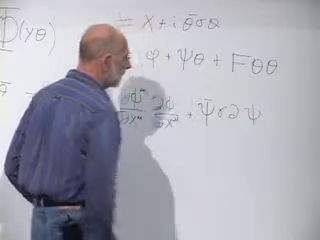
\includegraphics[width=0.76\textwidth]{lecture_09_figure_02.png}
\lectureframe{00:27:36.000}
\caption{上記のカイラル座標と成分展開は、スカラー、フェルミオン、補助項を扱っている。}
\end{figure}

\section{\texorpdfstring{\(d^2\theta\)}{d2-theta}積分が選び出すもの}

相互作用と質量は、正則関数\(W(\Phi)\)、すなわち超ポテンシャルから生じる：
\begin{equation}
S_W
=
\int d^4x
\left[
\int d^2\theta\,W(\Phi)
+\mathrm{h.c.}
\right].
\label{eq:l9-superpotential-action}
\end{equation}
カイラルな表式は独立な\(\bar\theta\)依存性を持たないので、それを4つの奇座標すべてについて積分するとゼロになる。代わりに\(d^2\theta\)積分はその\(\theta^2\)成分を選び出す。

一般関数を扱う前に組み合わせを理解するために、\(W(\Phi)=\Phi^n\)としよう。
\begin{equation}
(\phi+\sqrt2\,\theta\psi+\theta^2F)^n,
\end{equation}
において、ちょうど2つの\(\theta\)を得る方法は2通りある。単一の\(F\theta^2\)を選ぶか、2つのフェルミオン因子を選ぶかである。

\begin{classroomqa}
\audiencequestion{選ばれた1つの\(F\theta^2\)を含み、それ以外はスカラーのみである項はいくつあるか：\(n-1\)か\(n\)か？\lecturetimestamp{00:31:33}}
\lecturerresponse{\(n\)個ある。\(n\)個の因子のうちどれか1つが\(F\theta^2\)を与え、残りの\(n-1\)個の因子が\(\phi\)を与える。寄与は\(nF\phi^{n-1}\)である。}
\end{classroomqa}

\begin{classroomqa}
\audiencequestion{2つの因子が2つのフェルミオンを与える方法は何通りあるか？\lecturetimestamp{00:32:26}}
\lecturerresponse{\(\binom n2=n(n-1)/2\)通りの非順序な選択がある。グラスマン縮約が対応する\(\psi\psi\)項を固定する。}
\end{classroomqa}

したがって、講義の係数を省略した記法では、
\begin{equation}
\int d^2\theta\,\Phi^n+\mathrm{h.c.}
\;\leadsto\;
nF\phi^{n-1}
-\frac{n(n-1)}{2}\phi^{n-2}\psi\psi
+\mathrm{h.c.}
\label{eq:l9-power-extraction}
\end{equation}
ここに示された負号は標準的な規格化された展開とグラスマン規約に従うものであり、規約を変えれば表面的な符号は移動しうる。

\begin{classroomqa}
\audiencequestion{\(\theta\)を全く含まない項\(\phi^n\)はどうなったのか？\lecturetimestamp{00:33:10}}
\lecturerresponse{それは積の中に存在するが、\(d^2\theta\)がそれを捨てる。矢印は積分が\(\theta^2\)係数を選び出すことを意味しており、完全な表式の等式ではない。}
\end{classroomqa}

\begin{figure}[H]
\centering
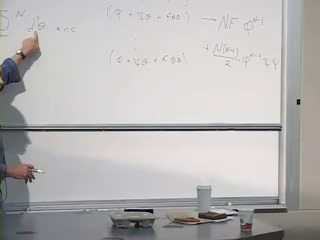
\includegraphics[width=0.82\textwidth]{lecture_09_figure_03.png}
\lectureframe{00:33:38.000}
\caption{繰り返された超場因子と、それらの2つの\(\theta\)成分を等置するのではなく抽出する含意矢印。}
\end{figure}

任意の係数を持つ冪を足し合わせると、組み合わせ因子が微分に変わる：
\begin{equation}
\int d^2\theta\,W(\Phi)+\mathrm{h.c.}
\;\leadsto\;
F W'(\phi)
-\frac12 W''(\phi)\psi\psi
+\mathrm{h.c.}
\label{eq:l9-W-components}
\end{equation}

\begin{classroomqa}
\audiencequestion{なぜフェルミオン項は\(\phi^{n-1}\)ではなく\(\phi^{n-2}\)を含むのか？\lecturetimestamp{00:36:32}}
\lecturerresponse{2つの因子がすでにフェルミオンを与えており、\(n-2\)個のスカラー因子が残る。係数は2階微分\(W''(\phi)\)の半分である。}
\end{classroomqa}

フェルミオン項は重要である：\(W''\)が定数のとき質量を与え、\(W''\)が\(\phi\)に依存するとき湯川相互作用を与える。しかし真空の解析には、補助項\(FW'\)が直接的な情報を担っている。

\section{補助場の消去}

\(F\)を含む項を集めると：
\begin{equation}
\mathcal L_F
=
F^\ast F
+F W'(\phi)
+F^\ast \overline{W'(\phi)}.
\label{eq:l9-LF}
\end{equation}
\(\partial_\mu F\)が存在しないので、完全なオイラー--ラグランジュ方程式
\begin{equation}
\partial_\mu
\frac{\partial\mathcal L}{\partial(\partial_\mu F)}
-
\frac{\partial\mathcal L}{\partial F}
=0
\end{equation}
は直ちに代数方程式に帰着する。\(F\)と\(F^\ast\)を独立変数として扱うと
\begin{align}
\frac{\partial\mathcal L_F}{\partial F}
&=F^\ast+W'(\phi)=0,
&
\frac{\partial\mathcal L_F}{\partial F^\ast}
&=F+\overline{W'(\phi)}=0,
\label{eq:l9-F-eom}
\end{align}
したがって
\begin{equation}
F^\ast=-W'(\phi),
\qquad
F=-\overline{W'(\phi)}.
\label{eq:l9-F-solution}
\end{equation}

\begin{figure}[H]
\centering
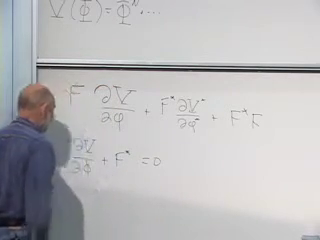
\includegraphics[width=0.82\textwidth]{lecture_09_figure_04.png}
\lectureframe{00:39:40.000}
\caption{完全な補助場の表式とその代数的運動方程式。黒板から遮蔽が取り除かれた後、両者が一緒に見える。}
\end{figure}

\begin{classroomqa}
\audiencequestion{その微分は、黒板に書かれた共役場ではなく\(\phi\)に関して取るべきか？\lecturetimestamp{00:41:21}}
\lecturerresponse{はい。その修正により式~\eqref{eq:l9-F-eom}の共役対が回復する：\(F^\ast=-W'(\phi)\)と\(F=-\overline{W'(\phi)}\)。}
\end{classroomqa}

式~\eqref{eq:l9-LF}に代入すると
\begin{equation}
\mathcal L_F\big|_{\mathrm{on\ shell}}
=-|W'(\phi)|^2.
\end{equation}
スカラーラグランジアンは運動エネルギーからポテンシャルエネルギーを引いた形をとるので、通常のスカラーポテンシャルは
\begin{equation}
\boxed{V(\phi,\phi^\ast)=|W'(\phi)|^2\ge0.}
\label{eq:l9-F-potential}
\end{equation}
この\(V\)は超ポテンシャルではない。\(W\)は正則な超空間関数のために、\(V\)は通常のポテンシャルエネルギーのために取っておく。

\subsection{2つの直接的な例}

厳密な従来の規格化では、
\begin{equation}
\begin{gathered}
W(\Phi)=\frac12m\Phi^2,\\
W'(\phi)=m\phi,
\qquad V=|m|^2|\phi|^2.
\end{gathered}
\label{eq:l9-quadratic-W}
\end{equation}
同じ項がフェルミオン質量
\(-\tfrac12m\psi\psi+\mathrm{h.c.}\)を与えるので、超対称性が破れる前にスカラー質量とフェルミオン質量は一致する。

\begin{equation}
W(\Phi)=\frac{g}{3}\Phi^3,
\end{equation}
に対して
\begin{equation}
\begin{gathered}
W'(\phi)=g\phi^2,
\qquad V=|g|^2|\phi|^4,\\
\mathcal L_{\mathrm{Yukawa}}
=-g\phi\psi\psi+\mathrm{h.c.}
\end{gathered}
\label{eq:l9-cubic-W}
\end{equation}
が得られる。四次スカラー頂点は二スカラー散乱を記述し、一方、湯川項はその超対称的な相棒である。

\section{2種類の真空}

真空は\(V\)の極小における定数場配置であり、その微分項は消える。式~\eqref{eq:l9-F-potential}は非負であるから、2つの場合が可能である。

\subsection{ゼロエネルギーの極小}

ある\(\phi_0\)が
\begin{equation}
W'(\phi_0)=0,
\end{equation}
を満たすならば
\begin{equation}
V(\phi_0)=0,
\qquad
\langle F\rangle=0.
\label{eq:l9-unbroken-F}
\end{equation}
真空は超対称的である。これは磁化が消えることの類似物である：どの補助成分も超空間の方向を選んでいない。

\subsection{持ち上げられた極小}

方程式
\begin{equation}
W'(\phi)=0
\label{eq:l9-F-flatness}
\end{equation}
が極小において同時解を持たないならば
\begin{equation}
V_{\min}>0,
\qquad
\langle F\rangle\neq0,
\label{eq:l9-broken-F}
\end{equation}
であり、超対称性は自発的に破れる。作用は超対称的であり続けるが、その最低エネルギー状態はそうではない。

\begin{figure}[H]
\centering
\includegraphics[width=0.88\textwidth]{lecture_09_figure_05.png}
\lectureframe{00:52:09.960}
\caption{黒板には正のポテンシャル、\(F\)方程式、そして真空条件が示されたままであり、対称な方程式と非対称な解とが区別されている。}
\end{figure}

秩序変数についての記述は、フェルミオン変換によって精密化できる：
\begin{equation}
\delta\psi_\alpha
=
i\sqrt2
(\sigma^\mu\bar\epsilon)_\alpha\partial_\mu\phi
+\sqrt2\,\epsilon_\alpha F.
\label{eq:l9-fermion-transformation}
\end{equation}
一様な真空では微分項は消える。もし
\(\langle F\rangle\neq0\)
ならば、超対称性はフェルミオンを非零の定数だけずらすので、真空は不変ではありえない。\editorialnote{式~\eqref{eq:l9-fermion-transformation}は、超場の成分が互いに回転し合うという講義の記述を明示する標準的な成分形である。}

同じ結論は超代数からも導かれる。静止系では、
\begin{equation}
\{Q_\alpha,Q_{\dot\alpha}^\dagger\}
=2\sigma^0_{\alpha\dot\alpha}H.
\end{equation}
真空期待値をとると、そのエネルギーは真空に作用する超電荷のノルムの和として表される：
\begin{equation}
E_0\ge0,
\qquad
E_0=0
\ \Longleftrightarrow\
Q_\alpha|0\rangle
=Q_{\dot\alpha}^\dagger|0\rangle=0.
\label{eq:l9-algebra-vacuum-energy}
\end{equation}
したがって、正の真空エネルギーと自発的超対称性の破れは、同じ剛直な超対称性の記述の表裏である。

\begin{center}
\begin{tikzpicture}[x=1.2cm,y=1.0cm,>=Latex]
  \draw[->] (-3,0) -- (-0.2,0) node[right] {\(\phi\)};
  \draw[->] (-2.8,-0.15) -- (-2.8,2.1) node[above] {\(V\)};
  \draw[thick,teal!75!black,domain=-2.5:-0.5,samples=60]
    plot (\x,{0.65*(\x+1.5)^2});
  \fill (-1.5,0) circle (2pt);
  \node[below] at (-1.5,0) {\(F=0\)};
  \draw[->] (0.4,0) -- (3.2,0) node[right] {\(\phi\)};
  \draw[->] (0.6,-0.15) -- (0.6,2.1) node[above] {\(V\)};
  \draw[thick,orange!85!black,domain=0.9:2.9,samples=60]
    plot (\x,{0.55*(\x-1.9)^2+0.65});
  \fill (1.9,0.65) circle (2pt);
  \draw[dashed] (0.6,0.65) -- (1.9,0.65);
  \node[below] at (1.9,0.65) {\(F\neq0\)};
\end{tikzpicture}
\end{center}

\editorialnote{最小の例は\(W=f\Phi\)であり、これに対して\(W'=f\)は決して消えず、\(V=|f|^2\)である。この一つの場の例には平坦なスカラー方向が存在する；現実的な安定な\(F\)項の破れは、通常、O'Raifeartaigh型の隠れたセクターのように、複数のカイラル場を用いて実現される。}

\section{破れた超対称性がもたらすもの}

\subsection{質量の分裂}

強磁性体の類推はここで再びスペクトルの言葉になる。弱い内部磁場は原子の同一性を壊すことなく原子準位を分裂させる。同様に、弱く伝達される超対称性の破れの秩序変数は、本来なら一つの超多重項に属するボソンとフェルミオンを分裂させる。

\begin{classroomqa}
\audiencequestion{超対称性によって互いに回転させられ、したがって真空がそれを破ると質量の縮退を失う粒子はどれか？ \lecturetimestamp{00:51:40}}
\lecturerresponse{ボソンとフェルミオンである。状態がそれらを関係づける変換を尊重しなくなれば、それらの質量は等しいままでいる必要はない。}
\end{classroomqa}

この分裂は\(\langle F\rangle\)単独によって生じるのではなく、破れを可視の場に伝える結合に依存する。それらの結合が弱ければ、可視の粒子は識別可能なままであり、分裂は大統一やプランクのスケールに比べて小さい。もし強ければ、類推は、巨大な磁場によって歪められて長く認識不能な物体となった原子に相当するであろう。

\subsection{ゴールドスティーノ}

通常の破れた生成子に対しては、\(J|0\rangle\)はボソン的なゴールドストーン状態を与える。超電荷はフェルミオン的であり、ボソン状態をフェルミオン状態に変える。真空はボソン的であると数えられるので、破れた超電荷はフェルミオン的なゼロエネルギー状態を創り出す：
\begin{equation}
Q_\alpha|0\rangle
\sim
|\widetilde G_\alpha,\mathbf k=0\rangle.
\label{eq:l9-goldstino}
\end{equation}
その伝播する継続は質量のないワイルフェルミオン、すなわちゴールドストーンフェルミオンまたはゴールドスティーノである。

\begin{classroomqa}
\audiencequestion{超対称性変換が真空を固定しないならば、それはどのような新しい状態を創り出すか？ \lecturetimestamp{00:53:24}}
\lecturerresponse{質量のないフェルミオンである。通常のゴールドストーン定理のパターンは保たれるが、フェルミオン的な生成子がボソン的な真空をゴールドスティーノに変える。}
\end{classroomqa}

したがって、剛直な自発的超対称性の破れには二つの不可避な兆候がある：
\begin{equation}
\boxed{
V_{\min}>0
\qquad\text{and}\qquad
\text{a massless goldstino}.
}
\label{eq:l9-rigid-breaking-signatures}
\end{equation}

\section{隠れたセクター}

原子と強磁性体を二つのセクターと呼ぶと有用である。強磁性体は秩序変数を発達させる；原子はそこから伝達される場だけを感じる。結合が弱いとき、原子を操作してもマグノンをほとんど励起せず、磁気媒体への直接的なアクセスはほとんど与えない。そのとき強磁性体は隠れており、その存在は小さなスペクトル分裂から推論される。

超対称模型の構築も同じ言葉を用いる。隠れたセクターの追加の場が非零の\(F\)項または\(D\)項の期待値を発達させる。媒介機構と呼ばれる相互作用がその破れを可視セクターに伝え、超対称パートナーのソフト質量を生成する。弱い伝達は、可視の理論がはるかに高い基礎スケールで近似的に超対称であり続けながら、低エネルギーで厳密なボソン--フェルミオン縮退を示さないことを説明する。

この構築は自動的ではない。追加の場、安定な破れの真空、そして制御された媒介機構が必要である。これが、講義が現実的な超対称性の破れを、最小模型の単一の不可避な帰結としてではなく、複雑でやや作為的であると述べる理由である。

\section{重力は両方の兆候を変える}

\subsection{真空エネルギーが源となる}

重力がなければ、すべてのエネルギーを定数分だけずらしても非重力実験は変わらない。重力があると、真空エネルギー密度は宇宙定数としてアインシュタイン方程式に入る。正の\(V_{\min}\)は加速膨張を駆動する。そのスケールが超対称パートナー質量に必要とされる素粒子物理のスケールと同程度であれば、生じる曲率は観測値より桁違いに大きくなるだろう。

\begin{classroomqa}
\audiencequestion{重力を含めると、正の非零真空エネルギーは世界に何をするのか？ \lecturetimestamp{01:00:40}}
\lecturerresponse{それは宇宙定数として働き、加速膨張を駆動する。通常の素粒子物理のスケールでは、その効果は耐え難いほど大きくなるだろう。}
\end{classroomqa}

局所超対称性、すなわち超重力は、正の二乗の公式を変える。目安として、標準的な\(N=1\) \(F\)項ポテンシャルは
\begin{equation}
\begin{aligned}
V_F={}&e^{K/M_P^2}
\left(
K^{i\bar j}D_iW\,D_{\bar j}\overline W
-\frac{3|W|^2}{M_P^2}
\right),\\
D_iW={}&\partial_iW+\frac{\partial_iK}{M_P^2}W.
\end{aligned}
\label{eq:l9-sugra-potential}
\end{equation}
である。負の項のため、超対称性の破れによる正のエネルギーは、原理的には部分的に相殺されうる。残りは小さな宇宙定数でありうる。

\editorialnote{この講義は意図的に模式的な補正のみを与え、プランク質量の配置について明示的に疑問を投げかけている。式~\eqref{eq:l9-sugra-potential}は、ケーラー・ポテンシャル\(K\)をもつカイラル多重項に対する従来の公式を記録している。ゲージ\(D\)項はさらに非負の寄与を加えるだろう。それは観測されている微小な値を説明するものではなく、それは宇宙定数問題として残る。}

\subsection{超ヒッグス機構}

第二の重力的効果は、偏極の数を数えることによって最も容易に理解される。質量をもつスピン\(j\)粒子は、その静止系で\(2j+1\)個のスピン状態をもつ。

\begin{classroomqa}
\audiencequestion{質量をもつスピン\(j\)粒子はいくつのスピン状態をもつか？ \lecturetimestamp{01:05:16}}
\lecturerresponse{\(2j+1\)。特に、質量をもつスピン1粒子は3つの状態をもつが、質量のないゲージボソンはヘリシティ\(+1\)と\(-1\)のみをもつ。}
\end{classroomqa}

この区別は運動学的である。質量をもつ粒子は静止系へブーストでき、その後スピンの向きを保ったまま新たな方向へ送り出せるので、すべての射影が存在しなければならない。質量のない粒子は追い越したり静止させたりできない。したがって、両端の2つのヘリシティのみを担いうる。

電弱ゲージ場に対して、
\begin{equation}
\underbrace{(+1,-1)}_{\text{massless vector}}
+
\underbrace{(0)}_{\text{Goldstone}}
\longrightarrow
\underbrace{(+1,0,-1)}_{\text{massive vector}}.
\label{eq:l9-higgs-count}
\end{equation}

\begin{classroomqa}
\audiencequestion{質量をもつ\(W\)や\(Z\)の縦偏極はどこから来るのか？ \lecturetimestamp{01:08:50}}
\lecturerresponse{ゴールドストーンボソンからである。それはゲージ場に吸収され、3状態の質量をもつスピン1表現を完成させる。}
\end{classroomqa}

重力には質量のないスピン2のグラビトンがある。その超対称パートナーは質量のないスピン\(\tfrac32\)のグラビティーノである。

\begin{classroomqa}
\audiencequestion{グラビトンのスピンは何であり、したがってその超対称パートナーのスピンは何か？ \lecturetimestamp{01:10:24}}
\lecturerresponse{グラビトンはスピン\(2\)をもつ。フェルミオン的パートナーは1/2だけ異なり、スピン\(3/2\)をもつ。}
\end{classroomqa}

質量のないグラビティーノはヘリシティ\(\pm\tfrac32\)をもつが、質量をもつグラビティーノは\(\pm\tfrac12\)ももたなければならない。ゴールドスティーノはまさにそれらの欠けた状態を供給する：
\begin{equation}
\begin{gathered}
\underbrace{\left(+\frac32,-\frac32\right)}_{\text{massless gravitino}}
\oplus
\underbrace{\left(+\frac12,-\frac12\right)}_{\text{goldstino}}\\
\Downarrow\\
\underbrace{\left(+\frac32,+\frac12,-\frac12,-\frac32\right)}_{\text{massive gravitino}}.
\end{gathered}
\label{eq:l9-super-higgs}
\end{equation}
これが超ヒッグス機構である。超対称性が局所的になると、ゴールドスティーノは吸収され、もはや独立な質量のない粒子として現れない。結果として生じるグラビティーノは重力的に相互作用し、それに対応して生成が難しい。

\section{話題の変更：なぜ\texorpdfstring{\(SU(5)\)}{SU(5)}なのか？}

超対称性の形式から、ここで大統一へと移る。標準模型のゲージ群は
\begin{equation}
G_{\mathrm{SM}}
=SU(3)_c\times SU(2)_L\times U(1)_Y.
\label{eq:l9-sm-group}
\end{equation}
である。その3つの因子はそれぞれ色、弱アイソスピン、弱ハイパーチャージを組織する。統一の問題は、この積が1つのより大きな単純群の残存部分群であるかどうか、すなわち、一見別々の粒子多重項とゲージ力が単一の構造の断片であるかどうかである。ここで展開される最小の候補は\(SU(5)\)である。

\subsection{群の要素と生成子}

\(U\in SU(N)\)に対して、
\begin{equation}
U^\dagger U=\mathbf1,
\qquad
\det U=1.
\label{eq:l9-SUN-def}
\end{equation}
第一の条件はユニタリー性であり、第二の条件は特殊の意味である。無限小要素を
\begin{equation}
U=\mathbf1+i\epsilon G+\mathcal O(\epsilon^2).
\label{eq:l9-infinitesimal-U}
\end{equation}
と書く。ユニタリー性は
\begin{equation}
G^\dagger=G,
\end{equation}
を要求し、
\begin{equation}
\det e^{i\epsilon G}
=e^{i\epsilon\operatorname{tr}G}=1
\end{equation}
は
\begin{equation}
\operatorname{tr}G=0.
\end{equation}
を要求する。したがって、生成子はトレースレスなエルミート行列である。

\(N\times N\)エルミート行列は\(N^2\)個の実パラメータを含む：\(N\)個の実対角成分と\(N(N-1)/2\)個の複素非対角成分である。トレースレス性が1つを取り除く。したがって
\begin{equation}
\dim SU(N)=N^2-1,
\qquad
\dim SU(5)=24.
\label{eq:l9-SU5-dimension}
\end{equation}
比較として、\(SU(2)\)は3つのパウリ生成子をもち、\(SU(3)\)は8つの色生成子をもつ。

\section{\texorpdfstring{\(SU(5)\)}{SU(5)}の内部の標準模型のブロック}

5次元空間を、弱い2次元ブロックとカラーの3次元ブロックに分ける：
\begin{equation}
\mathbf5=\mathbf2\oplus\mathbf3.
\end{equation}
埋め込まれた生成子は次の形をとる。
\begin{align}
T^a_L
&=
\begin{pmatrix}
\tfrac12\tau^a&0\\
0&0_{3\times3}
\end{pmatrix},
&& a=1,2,3,
\label{eq:l9-SU2-block}\\
T^A_c
&=
\begin{pmatrix}
0_{2\times2}&0\\
0&\tfrac12\lambda^A
\end{pmatrix},
&& A=1,\ldots,8.
\label{eq:l9-SU3-block}
\end{align}
パウリ行列\(\tau^a\)は弱い\(SU(2)\)を生成し、ゲルマン行列\(\lambda^A\)はカラー\(SU(3)\)を生成する。ブロックは重ならないので、この2つの部分群は可換である。

もう1つの対角生成子は各ブロック内で単位行列に比例するため、両方と可換である。基本表現では、便利な2倍ハイパーチャージの規約の1つは
\begin{equation}
T_Y^{(\mathbf5)}=
\operatorname{diag}
\left(
1,1,-\frac23,-\frac23,-\frac23
\right).
\label{eq:l9-hypercharge-generator}
\end{equation}
であり、そのトレースは消える：
\begin{equation}
1+1-3\left(\frac23\right)=0.
\end{equation}
共役な物質表現は反対の固有値をもつ：
\begin{equation}
Y_{\overline{\mathbf5}}
=
\operatorname{diag}
\left(
-1,-1,\frac23,\frac23,\frac23
\right),
\label{eq:l9-fivebar-hypercharge}
\end{equation}
これらは講義で物質の列に書かれた値である。全体の符号と規格化は規約であり、これらの成分は標準模型の規約
\begin{equation}
Q=T_3+\frac{Y}{2}.
\label{eq:l9-charge}
\end{equation}
を用いる。式~\eqref{eq:l9-SU2-block}--\eqref{eq:l9-hypercharge-generator}は
\begin{equation}
SU(3)_c\times SU(2)_L\times U(1)_Y
\subset SU(5).
\end{equation}
を示す。

3つの弱い生成子、8つのカラー生成子、1つのハイパーチャージ生成子で、\(24\)個の\(SU(5)\)生成子のうち\(12\)個を説明できる。\editorialnote{残りの12個は非対角な\(2\times3\)ブロックと\(3\times2\)ブロックを占める。それらのゲージボソンはクォーク型成分とレプトン型成分を互いに変換する。これが、続編で展開されるバリオン数とレプトン数を変える相互作用の構造的な起源である。}

\begin{classroomqa}
\audiencequestion{よく知られた部分群の生成子には、どのゲージ粒子が対応するのですか。\lecturetimestamp{01:31:05}}
\lecturerresponse{8個の\(SU(3)\)生成子は8個のグルーオンを与える。3個の\(SU(2)\)生成子は弱ゲージ場を与え、それらは電弱混合の後で\(W^\pm\)および\(Z\)光子系の一部となる。\(U(1)\)場はもう一方の中性結合を供給する。}
\end{classroomqa}

\section{左巻きの言葉で表した1世代}

第1世代に注目する。同じパターンがミューオン/チャーム/ストレンジ世代とタウ/トップ/ボトム世代でも繰り返される。すべての独立なワイル場を左巻きとして数えるのが最も経済的である。右巻き粒子は、その左巻き電荷共役場で表される：
\begin{equation}
Q_L=(u_L,d_L),\quad
L_L=(\nu_{eL},e_L),\quad
u^c_L,\quad d^c_L,\quad e^c_L.
\end{equation}
それらの多重度は
\begin{equation}
\underbrace{6}_{Q_L}
+
\underbrace{2}_{L_L}
+
\underbrace{3}_{u^c_L}
+
\underbrace{3}_{d^c_L}
+
\underbrace{1}_{e^c_L}
=15.
\label{eq:l9-fifteen-fields}
\end{equation}
である。

\editorialnote{最小標準模型には独立な右巻きニュートリノWeyl場が含まれないので、数は\(15\)である。この数え方だけでは、ニュートリノがMajorana粒子であることは主張されない。一重項\(\nu^c_L\)を加えると\(16\)個の場が得られ、自然に\(SO(10)\)を指し示すが、それは現在の\(SU(5)\)構成を超えている。}

5次元多重項は、無色の弱二重項成分を最初の2つの位置に置き、有色の弱一重項を最後の3つの位置に置かなければならない。

\begin{classroomqa}
\audiencequestion{提案された列には5つではなく6つの場が含まれるのではないか。\lecturetimestamp{01:36:14}}
\lecturerresponse{いいえ。最初の段階で書かれたアップクォークは消される。列はニュートリノ、電子、反ダウンクォークの3つのカラーコピーであり、全部で5つの成分である。}
\end{classroomqa}

これにより
\begin{equation}
\overline{\mathbf5}
=
\begin{pmatrix}
\nu_{eL}\\
e_L\\
d^c_{rL}\\
d^c_{gL}\\
d^c_{bL}
\end{pmatrix}.
\label{eq:l9-fivebar}
\end{equation}
\editorialnote{講義では当初これを単に5次元多重項と呼んでいる。標準的な全て左巻きの\(SU(5)\)記法では、その色とハイパーチャージの割り当ては、それが共役表現\(\overline{\mathbf5}\)であることを特定する。}
最初の2つの成分は\(SU(2)_L\)の下で変換するが、色の下では変換しない。最後の3つは色の下で反三重項として変換するが、弱一重項である。

\begin{classroomqa}
\audiencequestion{すべての場を左巻きで書いたとき、カラーをもつが弱い\(SU(2)_L\)量子数をもたないクォークはどれか。\lecturetimestamp{01:40:13}}
\lecturerresponse{右巻きクォークの電荷共役である。この5成分多重項では、電荷の検査により3つの反ダウン場\(d^c_{r,g,b}\)が選ばれる。}
\end{classroomqa}

式~\eqref{eq:l9-fivebar}の電荷は和がゼロになる：
\begin{equation}
0-1+\frac13+\frac13+\frac13=0.
\label{eq:l9-fivebar-charge-sum}
\end{equation}
これは、電荷演算子が\(SU(5)\)生成子のトレースレスな組み合わせであるために要求される。

\begin{classroomqa}
\audiencequestion{なぜ反アップクォークではなく反ダウンクォークが3つのカラーの位置を占めるのか。\lecturetimestamp{01:43:38}}
\lecturerresponse{ニュートリノと電子は合計電荷\(-1\)を与える。3つの反ダウンカラーは\(+1\)を与え、トレースをゼロにする。3つの反アップ場では合計電荷が正しくならない。}
\end{classroomqa}

残りの10個の左巻き場は
\begin{equation}
Q_L\;(6)
\oplus
u^c_L\;(3)
\oplus
e^c_L\;(1),
\end{equation}
であり、それらは反対称2階表現
\begin{equation}
\mathbf{10}\cong\wedge^2\mathbf5,
\qquad
\dim\wedge^2\mathbf5=\binom52=10.
\label{eq:l9-ten-preview}
\end{equation}
にちょうど収まる。それらの明示的な配置は次回の講義の課題である。すべての標準模型世代に対する数値的な適合
\begin{equation}
\overline{\mathbf5}\oplus\mathbf{10}
\end{equation}
は、\(SU(5)\)という考えが恣意的なラベルの付け替え以上のものであることを示す最初の顕著な証拠である。

\begin{classroomqa}
\audiencequestion{5と10が異なる表現であるなら、それらの粒子は相互作用できないのでしょうか。\lecturetimestamp{01:46:14}}
\lecturerresponse{いいえ。群変換は各既約表現の内部で作用するため、5の要素を10の要素へ直接回転させることはない。それでも、2つの組は共通のゲージボソンを放出・吸収することで相互作用でき、ヒッグス結合もそれらの場を結びつけ得る。}
\end{classroomqa}

\section{展望}

講義は、大きく異なるスケールにまたがる一つのパターンを追ってきた。回転不変性は原子準位を縮退させ、磁場の背景はそれを分裂させる。強磁性体はそのような背景を生み出しつつ、根底にある法則を対称なままにし、ギャップのないマグノンは非対称性が真空に宿ることを明らかにする。カイラル超対称理論では、補助場の期待値が秩序変数の役割を果たす：
\begin{equation}
\begin{aligned}
\langle F\rangle=0
&\quad\Longleftrightarrow\quad
\text{unbroken supersymmetry},\\
\langle F\rangle\neq0
&\quad\Longrightarrow\quad
\text{spontaneous breaking}.
\end{aligned}
\end{equation}
破れた真空は、剛直な超対称性において正のエネルギーを担い、超多重項を分裂させ、ゴールドスティーノを生み出す。弱い媒介は隠れたセクターを動機づけ、重力は真空エネルギーを宇宙論的問題に変え、ゴールドスティーノを質量をもつグラビティーノに吸収する。

締めくくりの\(SU(5)\)構成は、問いを完成させるのではなく新たな問いを始める。トレースレス・エルミートな\(5\times5\)生成子は標準模型のブロックを含み、最初の5つの物質場は
\((\nu_e,e^-,d^c_r,d^c_g,d^c_b)\)として正確に収まる。残りの10は反対称表現で待っている。この未完成の収まりこそが、大統一が本格的に始まるところである。
